\section{Thermodynamical tool}
\label{ch:thermtool}
Lucas

\subsection{Method of thermal analysis}

\subsubsection{Assumptions}
Lucas
\subsubsection{Leading equations}
The problem is modeled as a one-dimensional multilayer layup which can provide the accuracy needed or this stage of concept analysis as described in the assumptions. A description of the implementation of this model is given by Smith {Smith2011}. The model is illustrated in Figure \ref{fig:1dthermal}. The figure shows the different methods of heat transfer in the model. There is heat radiating away from the surface, convective heating or heat flux from the aerodynamic effects and heat conduction within the layers.

\begin{figure}[H]
	\centering
	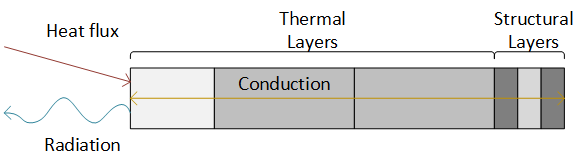
\includegraphics[width = 1.0\textwidth]{Figure/1dthermal.png}
	\caption{1D thermal model}
	\label{fig:1dthermal}
\end{figure}
\subsubsection{Input}
Lucas
\subsubsection{Output}
Suthes


\subsection{Verification & Validation}

\subsubsection{Verification}
Suthes
\subsubsection{Validation}



\subsection{Results per concept}



\subsection{Conclusion & recomendations}
